Un \textbf{\textit{stack de aplicaciones}} es una colección de software o tecnologías que se utilizan para crear una aplicación web. Las aplicaciones de una sola página \acrshort{spa} han crecido en popularidad ya que proporcionan una experiencia de usuario más fluida: llamadas de servidor livianas cambian lo que se muestra en la pantalla sin tener que actualizar toda la página. El resultado parece bastante ingenioso en comparación con la antigua forma de volver a cargar la página por completo. Esto provocó un aumento en los \glspl{framework} de \gls{frontend}, ya que gran parte del trabajo se realizó en el lado del cliente. Aproximadamente al mismo tiempo, aunque completamente sin relación, las bases de datos NoSQL también comenzaron a ganar popularidad. El término \textit{stack} fue popularizado por primera vez por LAMP Stack: Linux, Apache, MySQL y PHP. Linux es el sistema operativo, Apache actúa como el servidor HTTP, MySQL proporciona la base de datos relacional para manejar la información de la aplicación y PHP es el lenguaje de programación en el que se construye la aplicación. MERN es un paquete de software que significa MongoDB, Express.js, ReactJS y NodeJS. Juntos, estos programas gratuitos mejoran la simplicidad del proceso de desarrollo web. Las opciones son muchas, pero elegir una puede ser difícil.

% \section{LAMP}
% LAMP es un acrónimo de Linux, Apache, MySQL, PHP (Perl o Python), componentes de código abierto. Funciona como un paquete de programas que proporcionan una plataforma robusta para desarrollar e implementar aplicaciones y servidores basados en web. Durante años, ha sido la solución más efectiva para desarrollar aplicaciones web de nivel empresarial con personalización y flexibilidad mejoradas, de manera rentable. LAMP sigue siendo relevante, es muy atractivo para muchos usuarios porque es asequible y eficiente, ofreciendo una excelente alternativa a los paquetes de software comerciales. 
\subsection{Componentes}
\begin{itemize}
  \item Linux (sistema operativo)
  \item Apache (servidor web)
  \item MySQL (persistencia de datos)
  \item PHP (lenguaje de programación)
\end{itemize}

Derivados:

\begin{itemize}
  \item LAMP (con Perl o Python en lugar de PHP)
  \item LAMP (con MongoDB en lugar de MySQL)
  \item WAMP (Windows como SO)
  \item MAMP (Mac OS X como SO)
  \item XAMPP (Cualquier servidor OS + Perl o PHP + FTP)
  \item LAPP (PostgreSQL como base de datos)
\end{itemize}

\subsection{Beneficios}
Es utilizado por cientos de miles de empresas y, por lo tanto, su mantenimiento está muy bien respaldado. Con infinitos módulos, bibliotecas y complementos disponibles, puede ser adaptado a las necesidades de una empresa.\\[0.8cm]
Es posible controlar el servidor y decidir qué versiones y software se instalarán, por lo que no tiene que depender del navegador del cliente.
\subsection{Desventajas}
Debido a que es fácil de aprender, es posible caer en malas prácticas y crear aplicaciones basura. Comenzar con PHP, Python o Perl es fácil, pero dominarlo es difícil. Esto también es cierto para la seguridad en estas aplicaciones.

\section{MEAN/MERN}
En comparación con LAMP, el paquete de aplicaciones MEAN es bastante nuevo. Una de sus mayores diferencias es que MEAN no depende de un sistema operativo específico. Node.js se encarga de la ejecución del lado del servidor. MEAN Stack se recomienda especialmente para desarrolladores de JavaScript, ya que utiliza JavaScript en todos los niveles, tanto para el código del lado del cliente, así como el código del lado del servidor \cite{srinivasan}.
\vspace{0.8cm}

\subsection{Componentes MEAN}
\begin{itemize}
  \item MongoDB (base de datos)\\
  Una opción increíblemente popular en el mundo de la gestión de bases de datos NoSQL.
  \item Express.js (servidor)\\
  Para manejar las solicitudes de enrutamiento y proporcionar una API REST, o incluso puede usarse para generar el HTML final para ser utilizado por el \gls{framework} de \gls{frontend}.
  \item Angular.js / ReactJS (cliente)\\
  Es un potente \gls{framework} \gls{frontend}, utiliza un patrón de diseño Modelo-Vista-Controlador. ReactJS es una opción alternativa para el desarrollo \gls{frontend}, aunque React es simplemente una biblioteca, no un \gls{framework} MVC completo.
  \item Node.js (entorno del servidor)\\
  Permite al programador escribir el \gls{backend} de la aplicación en Javascript y ejecutarlo en la mayoría de los sistemas operativos modernos.
\end{itemize}

Derivados:

\begin{itemize}
  \item MERN (ReactJS en lugar de Angular.js)
  \item MEEN (Ember.js en lugar de Angular.js)
\end{itemize} 

\begin{figure}[H]
  \centering
  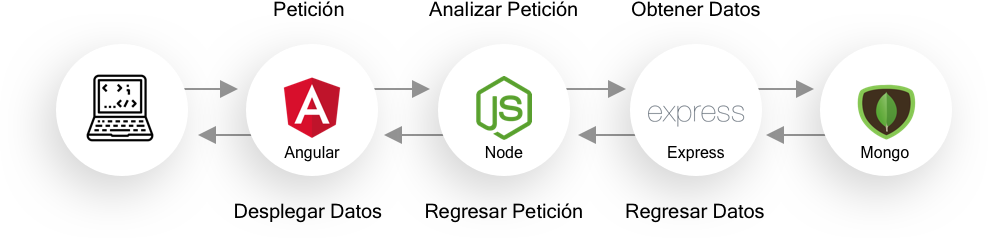
\includegraphics[width=1\textwidth]{mean}
  \caption{Flujo de información en MEAN Stack.}
\end{figure}

\subsection{Beneficios}
Usar JavaScript como el lenguaje de programación principal es una gran ventaja. Todo se puede configurar rápidamente y hacer en JavaScript, lo que hace que sea mucho más fácil encontrar desarrolladores, y los desarrolladores de LAMP generalmente también conocen JavaScript. Otra gran ventaja es la capacidad de crear fácilmente aplicaciones móviles o de escritorio, por ejemplo con \Gls{ionic}. El código y los componentes se pueden reutilizar o agregar fácilmente.

\subsection{Desventajas}
Muchas librerías y \glspl{framework} son bastante nuevos, y las nuevas versiones se lanzan rápidamente, por lo que mantener una aplicación puede ser una molestia. Dado que muchas tecnologías desaparecen después de unos años, la sostenibilidad puede convertirse en un problema. También es más difícil mantener una base de código limpia y seguir las mejores prácticas a medida que su aplicación crece. Además, debe confiar en el cliente y las tecnologías disponibles del cliente.

\newpage
\subsection{Base de datos NoSQL}
A pesar de la gran cantidad de bases de datos SQL, también hay una tendencia hacia NoSQL. Las bases de datos NoSQL permiten almacenar datos no estructurados y heterogéneos. La escalabilidad mejorada ha ayudado a aumentar su popularidad en mayor medida en el mercado actual. El escalado horizontal significa que la organización no tiene que preocuparse por la infraestructura subyacente. Las bases de datos NoSQL son una alternativa emergente a las bases de datos relacionales más utilizadas. Como su nombre lo indica, no reemplaza completamente a SQL, sino que lo complementa de tal manera que puedan coexistir.
\vspace{0.8cm}

\begin{table}[H]
  \renewcommand{\arraystretch}{1.5}
  \centering
  \scriptsize
  \begin{tabular}{ |p{2cm}||p{5cm}|p{5cm}|  }
    \hline
      & SQL
      & NoSQL \\
    \hline
    Tipo
      & Relacional
      & Distribuido \\
    \hline
    Datos
      & Datos estructurados almacenados en tablas 
      & Datos no estructurados almacenados en archivos JSON \\
    \hline
    Esquema 
      & Estático o predefinido
      & Dinámico \\
    \hline
    Escalable 
      & Vertical
      & Horizontal \\
    \hline
    Consultas
      & Adecuado para consultas complejas 
      & Lenguaje de consulta no estructurado \\
    \hline
    Flexible
      & Esquema rígido ligado a la relación 
      & Esquema adecuado para almacenamiento jerárquico \\
    \hline
    Elasticidad
      & Requiere tiempo de inactividad en la mayoría de los casos 
      & Automática, no requiere interrupción \\
    \hline
  \end{tabular}
  \caption{Comparativa SQL y NoSQL}
\end{table}
\vspace{0.8cm}

El concepto de NoSQL se desarrolló hace mucho tiempo, pero fue después de la introducción de la base de datos como servicio (DBaaS) que obtuvo un reconocimiento destacado. Debido a la alta escalabilidad proporcionada por NoSQL, fue visto como un importante competidor del modelo de base de datos relacional. A diferencia de las bases de datos relacionales (RDB), las bases de datos NoSQL están diseñadas para escalar fácilmente a medida que crecen. La mayoría de los sistemas NoSQL han eliminado el soporte multiplataforma y algunas características adicionales innecesarias de RDBMS, haciéndolos mucho más livianos y eficientes que sus contrapartes RDMS.


\subsection{Orientado a documentos}
El concepto principal de una base de datos orientada a documentos es que el documento contiene grandes cantidades de datos que pueden estar disponibles de manera útil. Se puede acceder a estos documentos como un directorio regular en el que puede tener diferentes colecciones y cada colección tiene documentos que contienen la información deseada. Además, cada colección puede tener colecciones internas. Puede tener un árbol completo de documentos, sin embargo, esta práctica no se recomienda y debe evitar tener más de tres niveles de anidamiento. 
\vspace{0.8cm}

Las bases de datos NoSQL no son necesariamente bases de datos relacionales. Los datos no son representados en términos de filas y columnas de tablas. En MongoDB, los datos se visualizan como objetos o documentos. Esto ayuda a un programador a evitar una capa de traducción, por lo que no es necesario convertir o asignar los objetos con los que trata el código en tablas relacionales. Dichas traducciones se denominan capas de Mapeo Relacional de Objetos (ORM).
\begin{figure}[H]
  \centering
  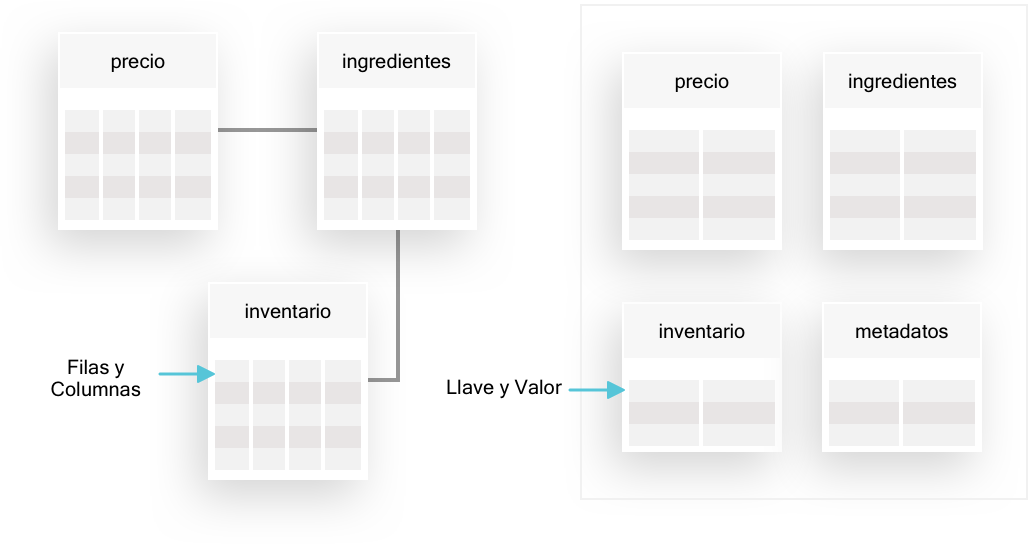
\includegraphics[width=1\textwidth]{sql-nosql}
  \caption{Diagrama que representa las diferencias clave entre la base de datos SQL y las bases de datos NoSQL.}
\end{figure}

\subsection{Angular/React}
Angular o React, proporcionan la interfaz de usuario reactiva de una aplicación. Utilizan componentes, son reactivos porque el usuario recibe cambios inmediatos cuando interactúa con la aplicación y, por lo general, se ejecutan dentro del navegador de un usuario (aunque ambos son isomórficos, capaces de ejecutarse en un servidor).
\vspace{0.8cm}

\begin{table}[H]
  \renewcommand{\arraystretch}{1.5}
  \centering
  \scriptsize
  \begin{tabular}{ |p{2cm}||p{5cm}|p{5cm}|  }
    \hline
      & Angular
      & React \\
    \hline
    Desarrollador
      & Google
      & Facebook \\
    \hline
    Definición
      & Framework
      & Librería \\
    \hline
    Modelo de plantilla
      & HTML + Typescript
      & JSX + Javascript \\
    \hline
    Flujo
      & 2 vías
      & Unidireccional \\
    \hline
    DOM
      & Regular
      & Virtual \\
    \hline
    Lógica/Estado de la aplicación
      & Services
      & Flux/Redux \\
    \hline
  \end{tabular}
  \caption{Características de Angular.js y React.js}
\end{table}
\vspace{0.8cm}

Angular es un framework con muchas herramientas integradas, para hacer solicitudes HTTP, enrutamiento y navegación, animaciones y otros. Se basa en módulos que son componentes y servicios.
\vspace{0.8cm}

React es una biblioteca de Javascript, que se puede usar para crear nuevas aplicaciones o para integrarla con una aplicación existente. React se basa en componentes pequeños y reutilizables, que administran su propio estado y luego los componen para crear interfaces de usuario complejas. Incluso si React no es tan complejo como Angular, con muchas cosas integradas, hay muchas bibliotecas que se pueden agregar para tener enrutadores (react-router) y solicitudes HTTP (axios), manejo de estado (react-redux) entre otras más. Esto lo hace portátil y fácil de incorporar en cualquier entorno.

\newpage
\section{FERN}
Firebase es una plataforma propiedad de Google que tiene como objetivo proporcionar un enfoque completo para un rápido desarrollo web y móvil. En resumen, le permite centrarse en las partes frontales de la aplicación. Se completa con una base de datos NoSQL, alojamiento, almacenamiento de archivos, procesamiento del lado del servidor para cosas que deben protegerse de la interfaz y un sistema de autenticación, que junto a módulos de desarrollo \textit{frontend} como React.js, proporcionan todo lo necesario para crear aplicaciones web pequeñas y medianas.
\vspace{0.8cm}

\subsection{Componentes FERN}
\begin{itemize}
  \item Firebase (base de datos)
  \item Express.js (servidor)
  \item React.js (cliente)
  \item Node.js (entorno del servidor)
\end{itemize}
\begin{figure}[H]
  \centering
  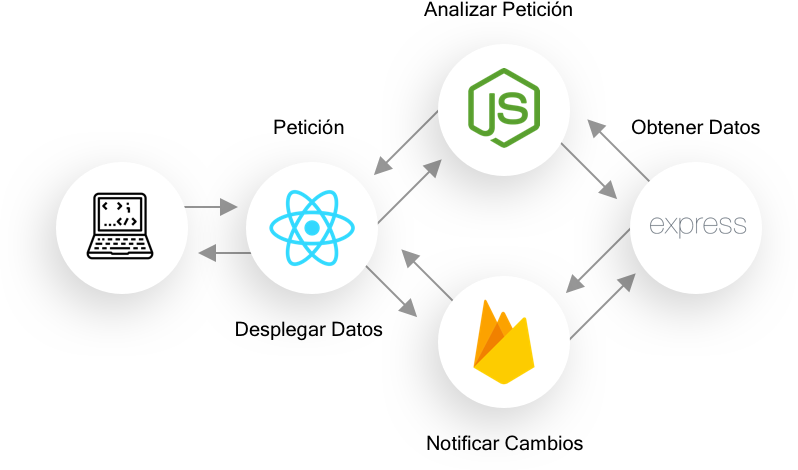
\includegraphics[width=0.8\textwidth]{fern}
  \caption{Flujo de información en FERN Stack.}
\end{figure}

\subsection{Cloud Firestore}
Firestore es una bases de datos orientada a documentos, toda la información se guarda en colecciones como JSON, principalmente diseñada para almacenar, recuperar y administrar información orientada a documentos, también conocida como datos semiestructurados.
\vspace{0.8cm}

La escalabilidad es completamente automática, lo que significa que no es necesario compartir sus datos en varias instancias. Los cargos de Cloud Firestore se basan en las operaciones realizadas en su base de datos (lectura, escritura, borrado), ancho de banda y almacenamiento. Admite límites de gasto diario para proyectos de Google App Engine, para garantizar que no exceda los costos con los que el usuario se sienta cómodo.
\begin{figure}[H]
  \centering
  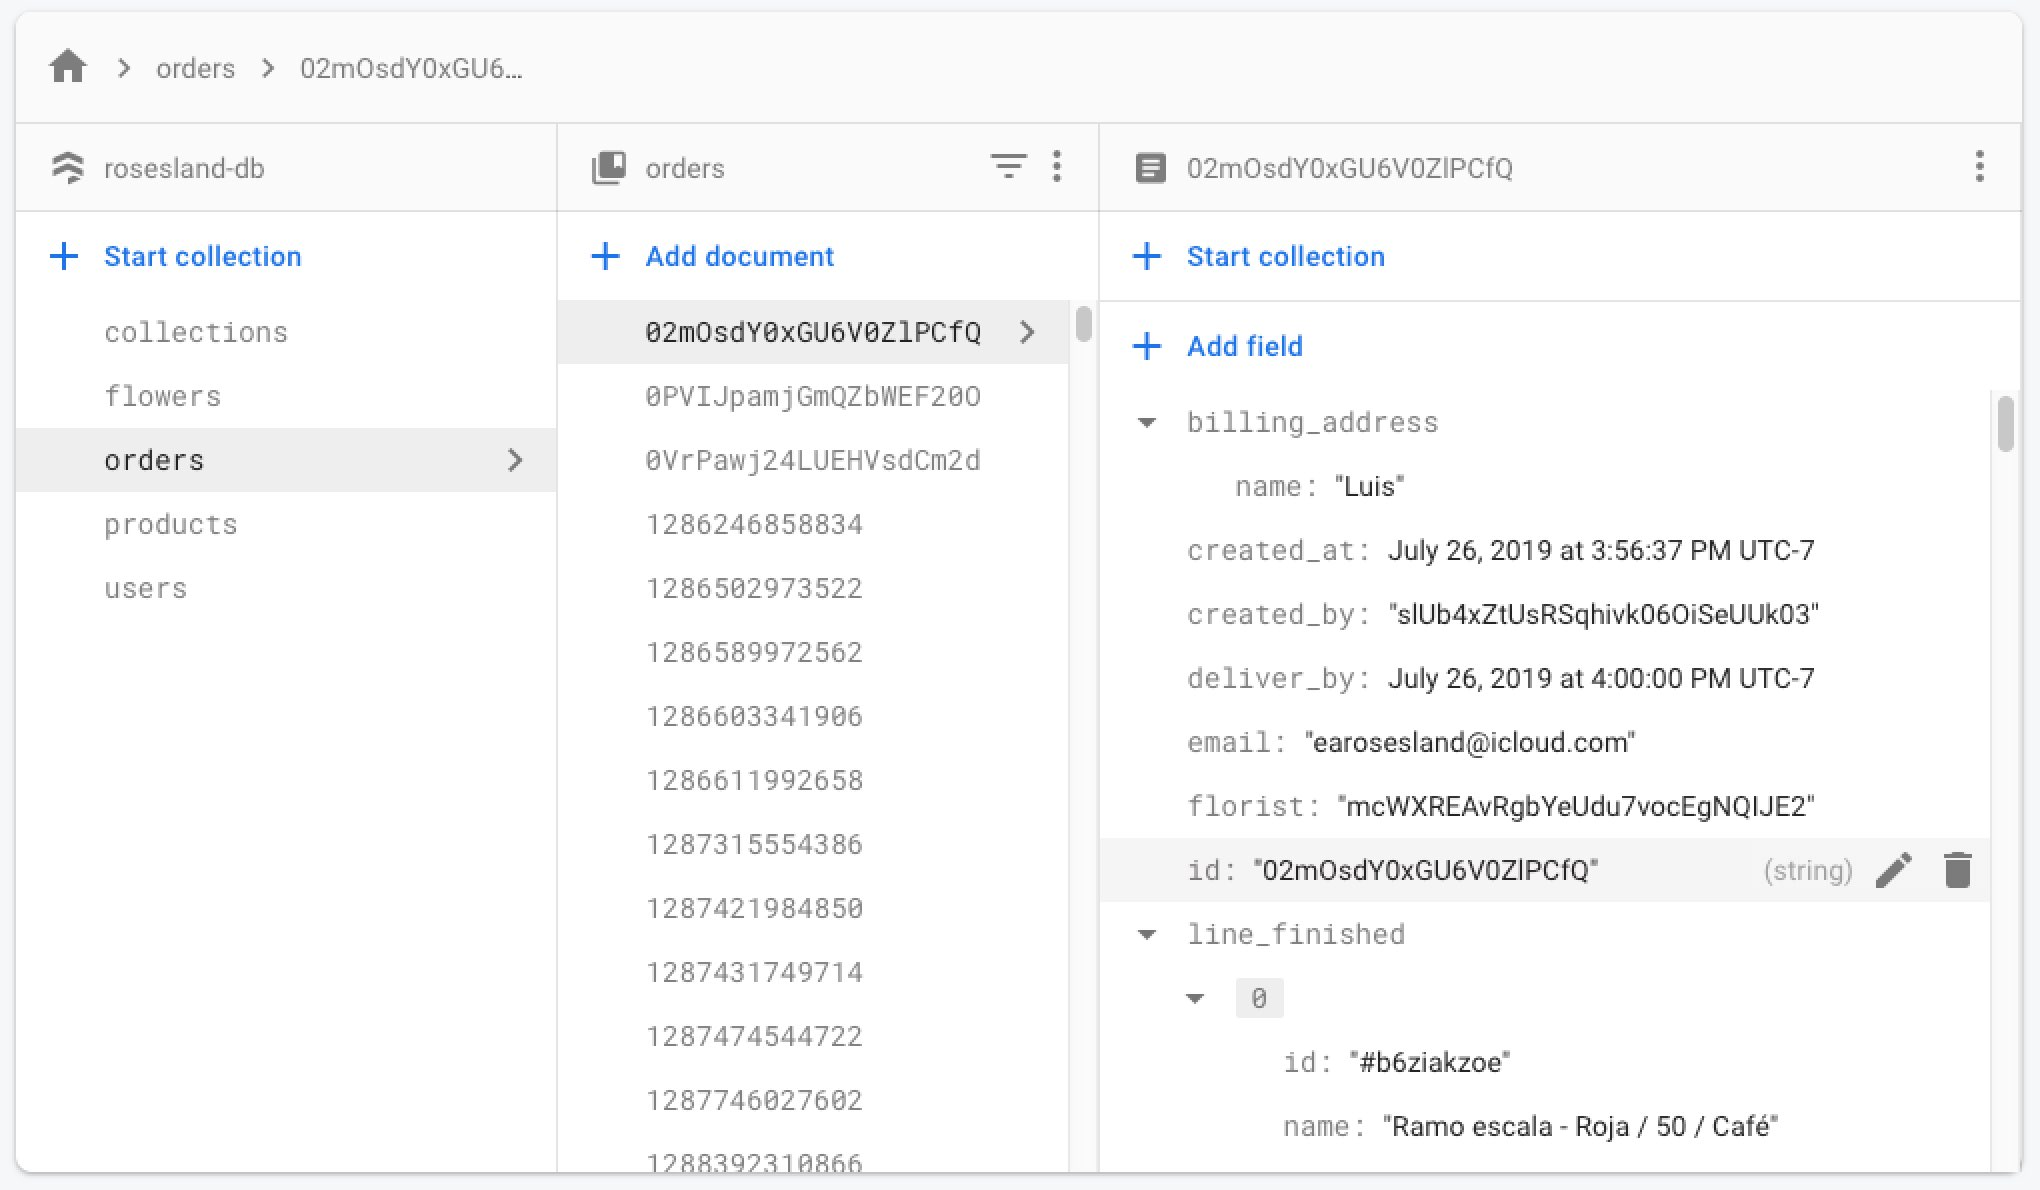
\includegraphics[width=0.9\textwidth]{firestore}
  \caption{Colección de Firestore con sus documentos internos.}
\end{figure}

\subsection{Node.js}
Node.js es un entorno multiplataforma de código abierto para ejecutar código JavaScript del lado del servidor. El entorno de tiempo de ejecución de Node.js incluye todo lo que necesita para ejecutar un programa escrito en JavaScript. 
\vspace{0.8cm}

Node.js surgió cuando los desarrolladores originales de JavaScript lo extendieron de algo que solo podía ejecutar en el navegador a algo que podría ejecutar en su máquina como una aplicación independiente. Ahora puede hacer mucho más con JavaScript que simplemente hacer que los sitios web sean interactivos. JavaScript ahora tiene la capacidad de hacer cosas que otros lenguajes de secuencias de comandos como Python pueden hacer. Tanto su navegador JavaScript como Node.js se ejecutan en el motor de tiempo de ejecución JavaScript V8. Este motor toma su código JavaScript y lo convierte en un código de máquina más rápido. El código de máquina es un código de bajo nivel que la computadora puede ejecutar sin necesidad de interpretarlo primero.
\vspace{0.8cm}

\begin{figure}[H]
  \centering
  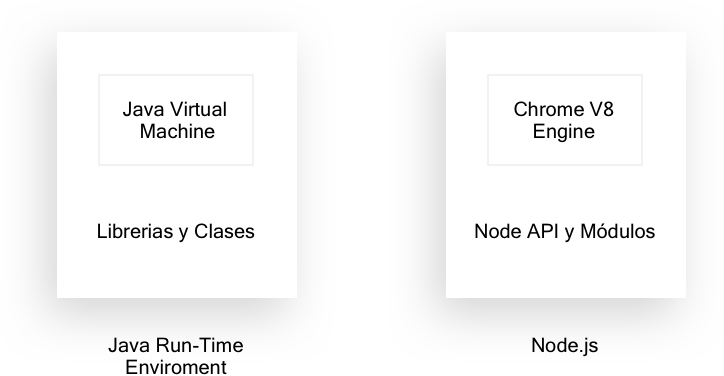
\includegraphics[width=0.8\textwidth]{node}
  \caption{Analogía Node.js con Java.}
\end{figure}
% \vspace{0.8cm}

\subsubsection{Motor V8 de Google Chrome}
Node.js utiliza el motor de ejecución ultra rápido V8 de Google Chrome. Hasta el lanzamiento de Chrome, la mayoría de los navegadores leían JavaScript de manera ineficiente: el código se leía e interpretaba poco a poco. Tomó mucho tiempo leer JavaScript y convertirlo a lenguaje máquina para que el procesador pudiera entenderlo. 
\vspace{0.8cm}

El motor V8 de Google Chrome funciona completamente diferente. Está altamente optimizado y lleva a cabo lo que llamamos compilación JIT (Just In Time). Transforma rápidamente el código JavaScript en lenguaje máquina.
\vspace{0.8cm}

\begin{table}[H]
  \renewcommand{\arraystretch}{1.5}
  \centering
  \scriptsize
  \begin{tabular}{ |p{2cm}||p{5cm}|p{5cm}|  }
    \hline
        Navegador
      & Motor de renderizado / diseño
      & Motor de secuencias de comandos \\
    \hline
        Chrome
      & Blink (C++)
      & V8 (C++) \\
    \hline
    \hline
        Mozilla Firefox
      & Gecko (C++)
      & SpiderMonkey (C/C++) \\
    \hline
    \hline
        IE Edge
      & EdgeHTML (C++)
      & Chakra JavaScript engine (C++) \\
    \hline
    \hline
    Opera
      & Blink (C++)
      & V8 (C++) \\
    \hline
    Internet Explorer
      & Trident (C++)
      & Chakra JScript engine (C++) \\
    \hline
  \end{tabular}
  \caption{Motores de renderizado y secuencias de comandos}
\end{table}
\vspace{0.8cm}


\subsection{El ecosistema NPM}
NPM (Node Package Manager) es el administrador de paquetes predeterminado para Node.js. Paquete es un término utilizado por npm para denotar herramientas que los desarrolladores pueden usar para sus proyectos \cite{goalkicker-node}. Se instala en el sistema con la instalación de Node.js. Los paquetes y módulos necesarios en un proyecto Node se instalan utilizando \textit{npm}.
\vspace{0.8cm}

NPM consta de tres componentes:
\begin{enumerate}
  \item Sitio web
  \item Registro
  \item CLI
\end{enumerate}
\subsubsection{Sitio web}
El sitio web oficial de npm es https://www.npmjs.com/. Con este sitio web puede encontrar paquetes, ver documentación, compartir y publicar paquetes.
\subsubsection{Registro}
El registro npm es una gran base de datos que consta de más de medio millón de paquetes. Los desarrolladores descargan paquetes del registro npm y publican sus paquetes en el registro.
\subsubsection{CLI (interfaz de línea de comando)}
Esta es la línea de comando que ayuda a interactuar con el npm para instalar, actualizar y desinstalar paquetes y administrar dependencias.
\subsection{Comandos NPM}
Npm tiene muchos paquetes que puedes usar en una aplicación para que su desarrollo sea más rápido y eficiente. Instalar módulos usando NPM no representa un gran problema. Hay una sintaxis simple para instalar cualquier módulo Node.js:
\vspace{0.8cm}

% \begin{verbatim}
%   npm install nombre-del-paquete
%   ejemplo: npm install express
% \end{verbatim}
\begin{lstlisting}[language=HTML]
  npm install nombre-del-paquete
  ejemplo: npm install express
\end{lstlisting}
% \lstinputlisting[style=ES6, caption=Comandos para instalar paquete con NPM]{code/npm.txt}

\subsection{Express.js}
Escribir un servidor web completo a mano en Node.js directamente no es tan fácil, ni es necesario, Express.js es un paquete de aplicación web minimalista y extensible creado para el ecosistema Node.js. Permite crear un servidor web legible, flexible y fácil de mantener.
\vspace{0.8cm}

Express.js le permite definir rutas, especificaciones de qué hacer cuando llega una solicitud HTTP que coincide con un patrón determinado. La especificación coincidente se basa en expresiones regulares (regex) y es muy flexible, como la mayoría de los otros entornos de aplicaciones web. La parte de qué hacer es solo una función que recibe la solicitud HTTP analizada.
\vspace{0.8cm}

Express.js analiza la URL de solicitud, encabezados y parámetros. En el lado de la respuesta, tiene, como se esperaba, toda la funcionalidad requerida por las aplicaciones web. Esto incluye la configuración de códigos de respuesta, configuración de \glspl{cookie}, envío de encabezados personalizados, etc. Además, puede escribir middleware Express, piezas de código personalizadas que se pueden insertar en cualquier ruta de procesamiento de solicitud/respuesta para lograr una funcionalidad común como el registro, la autenticación, entre otras.
\vspace{0.8cm}


\lstinputlisting[style=ES6, caption=Simple aplicación Express.js]{code/express.js}

\subsection{React.js}
React es una biblioteca de JavaScript declarativa, eficiente y flexible creada en 2013 por el equipo de desarrollo de Facebook. React quería que las interfaces de usuario fueran más modulares (o reutilizables) y más fáciles de mantener. Según el sitio web de React, se utiliza para \textit{construir componentes encapsulados que administran su propio estado, y unirlos para crear interfaces de usuario complejas}. React es una biblioteca JavaScript que permite componer interfaces de usuario complejas a partir de piezas de código pequeñas y aisladas llamadas \textit{componentes}.
\vspace{0.8cm}

En términos generales, al crear aplicaciones con ReactJS, se crean componentes que corresponden a distintos elementos de una interfaz de usuario. Después se organizan estos elementos dentro de componentes de orden superior que definen la estructura de la aplicación. Es importante destacar que cada componente en una aplicación React se rige por principios estrictos de gestión de datos. Interfaces avanzadas comúnmente involucran datos complejos y manejo de estado. ReactJS es limitado y tiene como objetivo darnos las herramientas para poder anticipar cómo se verá una aplicación con un conjunto de circunstancias dado.

\subsection{Componentes React}
Un componente es una pequeña parte de la interfaz de usuario. Todas las piezas reutilizables de una página web se abstraen en estos elementos. Son similares, en conceptos, a cosas como \glspl{widget} y módulos. React se define a sí mismo como una biblioteca para construir interfaces de usuario. Como tal, cuando se piensa en una interfaz de usuario, se debe pensar en ella en términos de los componentes más pequeños posibles que se puedan definir. La razón por la que existe este paradigma es para disminuir el acoplamiento (cuánto dependen los unos de los otros) y aumentar la cohesión (qué tan bien funcionan juntas las diferentes cosas).
\vspace{0.8cm}

Cada uno de estos fragmentos es un bloque de código independiente y reutilizable, que divide la interfaz de usuario en partes más pequeñas. Incluyen código que define cómo se crean los elementos en el \acrshort{dom} y cómo los usuarios pueden interactuar con ellos. Los componentes se pueden definir únicamente en JavaScript o se pueden definir en un superconjunto (o variación extendida) de JavaScript llamado JSX, que se explica en temas posteriores.
\vspace{0.8cm}

\begin{figure}[H]
  \centering
  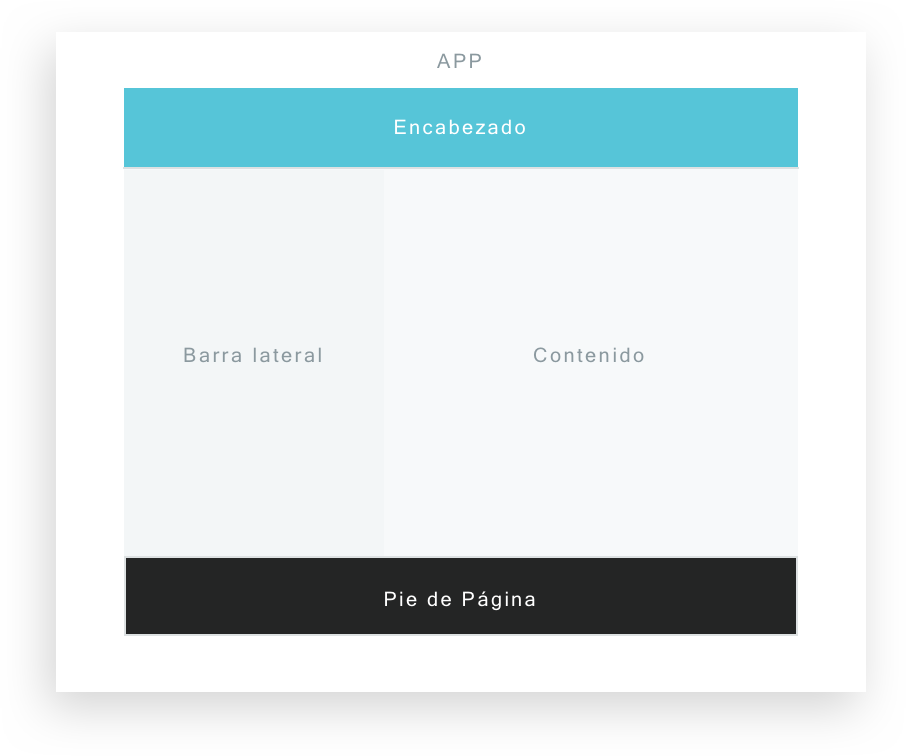
\includegraphics[width=0.8\textwidth]{components}
  \caption{Componentes principales de una página web. (Fuente: Elaboración propia)}
\end{figure}
En primer lugar, hay un elemento principal llamado componente APP. Este componente de la aplicación contiene cuatro fragmentos secundarios o se divide en cuatro componentes:
\begin{enumerate}
  \item Encabezado
  \item Barra lateral
  \item Contenido
  \item Pie de página
\end{enumerate}
La función de cada componente se manejará independientemente con otros componentes. Cada componente es una pieza reutilizable, y se puede pensar en cada componente de forma aislada.
\vspace{0.8cm}

Dentro de un componente, tendremos subcomponentes o componentes dentro de un componente padre. Esos serán reutilizables también. En pocas palabras, un componente es una clase o función de JavaScript que opcionalmente acepta entradas, es decir, propiedades (props) y devuelve un elemento que describe cómo debería lucir una sección de la interfaz de usuario.
\vspace{0.8cm}

\lstinputlisting[style=ES6, caption=Ejemplo de página con componentes ReactJS]{code/react-example.js}

\subsection{DOM Virtual}
En el desarrollo web de software, \acrshort{dom} significa Modelo de Objeto de Documento (Document Object Model) y representa la estructura de los elementos en una página web. El HTML DOM se construye como un árbol de objetos.

Algunas bibliotecas de JavaScript, como jQuery, manipulan los elementos DOM directamente, cambiando sus atributos, agregando o eliminando componentes. Sin embargo, en lugar de cambiar el DOM directamente, React usa un DOM virtual, que es una replicación virtual del árbol DOM actual. En consecuencia, React puede manipular el DOM virtual innumerables veces y comparar su estado con el DOM real. De esta manera, React sabe exactamente qué elemento cambió y luego actualiza solo ese elemento específico en la pantalla.

Detrás de escena, React hace un gran trabajo para editar y volver a \gls{renderizar} eficientemente el DOM cuando algo en la interfaz necesita cambiar. Este enfoque le brinda al desarrollador una gran flexibilidad y sorprendentes ganancias de rendimiento porque ReactJS calcula con anticipación qué cambios se deben realizar en el DOM y actualiza los árboles DOM en consecuencia. De esta manera, ReactJS evita las costosas operaciones DOM y realiza actualizaciones de manera eficiente \cite{stefanov}.


\newpage
\section{Preprocesamiento}
\subsection{ES5/ES6}
ES5 (ES significa ECMAScript) es básicamente `JavaScript normal'. La quinta actualización de JavaScript, ES5 se finalizó en 2009. Ha sido compatible con todos los principales navegadores durante muchos años. \\[0.8cm]
ES6 es una nueva versión de JavaScript que agrega algunas buenas adiciones sintácticas y funcionales. Se finalizó en 2015. ES6 es casi totalmente compatible con todos los navegadores principales. Pero pasará algún tiempo hasta que las versiones anteriores de los navegadores web estén fuera de uso. Por ejemplo, Internet Eyplorer 11 no es compatible con ES6, pero tiene aproximadamente el 8\% de uso de mercado de navegadores.\\[0.8cm]
Para aprovechar los beneficios de ES6 hoy, se tienen que hacer que hacer algunos procedimientos para que funcione en tantos exploradores de internet como sea posible:
\begin{enumerate}
  \item Se debe preprocesar el código para que una gama más amplia de navegadores entiendan nuestro JavaScript. Esto significa convertir ES6 JavaScript en ES5 JavaScript.
  \item Tenemos que incluir un `shim' o `polyfill' que brinde una funcionalidad adicional agregada en ES6 que un navegador puede o no tener.
\end{enumerate}
\subsubsection{JSX}
JSX es una extensión de sintaxis similar a XML para ECMAScript sin ninguna semántica definida. NO está destinado a ser implementado por motores o navegadores. NO es una propuesta para incorporar JSX en la propia especificación ECMAScript. Está destinado a ser utilizado por varios preprocesadores (transpiladores) para transformar estos tokens en ECMAScript estándar.
\subsubsection{BabelJS}
BabelJS es un transpilador de JavaScript que transpila nuevas características ES6 al antiguo estándar ES5. Con esto, las funciones se pueden ejecutar en navegadores antiguos y nuevos, sin problemas. \\[0.8cm]
\textbf{El preprocesador BabelJS} convierte la sintaxis de JavaScript moderno en un formulario, que los navegadores más antiguos pueden entender fácilmente. Por ejemplo, const y let se convertirán en var, la función flecha se convierte en una función normal manteniendo la funcionalidad igual en ambos casos.
\subsubsection{Sass (Syntactically Awesome Style Sheets)}
Sass es un preprocesador de CSS, que ayuda a reducir la repetición con CSS y ahorra tiempo. Es un lenguaje de extensión CSS más estable y potente que describe el estilo de una página estructuralmente. Sus principales atributos son:
\begin{enumerate}
  \item Es un súper conjunto de CSS, lo que significa que contiene todas las características de CSS y es un preprocesador de código abierto, codificado en Ruby.
  \item Proporciona algunas características, que se utilizan para crear hojas de estilo que permiten escribir código más eficiente y fácil de mantener.
\end{enumerate}
\subsubsection{Webpack}
Webpack es un empaquetador de módulos. Webpack toma un archivo de entrada, encuentra todos los archivos de los que depende y genera un archivo que contiene todo el código de una aplicación. Con él es posible importar archivos CSS e imágenes directamente a JavaScript. Se puede compilar CoffeeScript, TypeScript, SASS y LESS. También es capaz de compilar la sintaxis de ES6 en JavaScript amigable para el navegador. En otras palabras, Webpack toma diferentes archivos (como CSS, JS, SASS, JPG, SVG, PNG, etc.) y los combina en paquetes, un paquete separado para cada tipo de archivo.

\newpage
\section{Control de versiones}
Hoy en día no es prudente empezar un proyecto web sin una estrategia de respaldo. Debido a que los datos son efímeros y se pueden perder fácilmente, por ejemplo, a través de un cambio de código erróneo o un fallo catastrófico de disco, es aconsejable mantener un archivo de todo el trabajo.\\[0.8cm]
Para proyectos de texto y código, la estrategia de respaldo generalmente incluye control de versiones, o seguimiento y administración de revisiones.  Dado su papel fundamental, el control de versiones es más efectivo cuando se adapta a los hábitos y objetivos de trabajo del equipo del proyecto.\\[0.8cm]
En su forma más simple, un sistema de control de versiones proporciona un principio básico y un método para almacenar archivos y cambios realizados en ellos. Esto se logra mediante el uso de un repositorio. El repositorio contiene la versión más reciente de cada archivo y el historial de cambios que ha llevado a esa representación. Por lo general, cada cambio incluye información adicional, como el autor y una breve descripción.
\subsection{Git}
Git es un software de control de versiones distribuido particularmente potente, flexible y de bajo costo que hace que el desarrollo colaborativo sea un placer. \\[0.8cm]
La principal diferencia entre Git y cualquier otro versionador es la forma en que Git piensa acerca de sus datos. Conceptualmente, la mayoría de los otros sistemas almacenan información como una lista de cambios basados en archivos. Estos sistemas (CVS, Subversion, Perforce, Bazaar, etc.) piensan en la información que mantienen como un conjunto de archivos y los cambios realizados en cada archivo a lo largo del tiempo. Git no piensa ni almacena sus datos de esta manera. En cambio, Git piensa en sus datos más como un conjunto de instantáneas de un mini sistema de archivos. Cada vez que confirma o guarda el estado de su proyecto en Git, básicamente toma una fotografía de cómo se ven todos sus archivos en ese momento y almacena una referencia a esa instantánea. Para ser eficiente, si los archivos no han cambiado, Git no almacena el archivo nuevamente, solo un enlace al archivo idéntico anterior que ya ha almacenado. \\[0.8cm]
\begin{figure}[H]
  \centering
  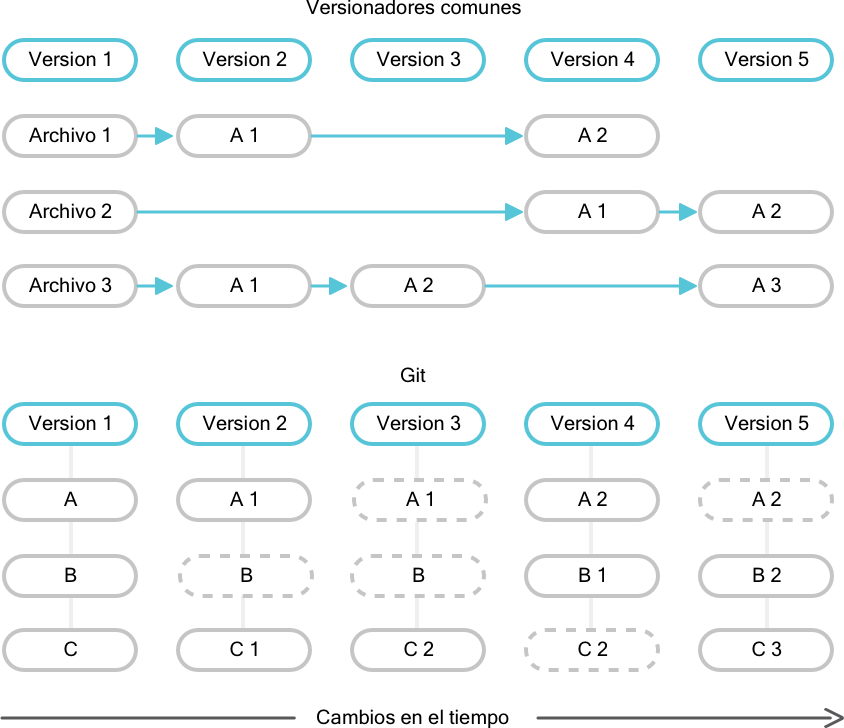
\includegraphics[width=0.9\textwidth]{git}
  \caption{Diferencias entre controladores de versiones. (Fuente: Elaboración propia)}
\end{figure}